For simplicity, the algorithms considered in this paper will be presented in a
tree-independent context, as in \citet{curtin2013tree}, but the only type of
tree we will consider is the cover tree \citep{langford2006}, and the only type
of traversal we will consider is the cover tree pruning dual-tree traversal,
which we will describe later.

As we will be making heavy use of trees, we must establish notation \citep[taken
from][]{curtin2013tree}.  The notation we will be using is defined in Table
\ref{tab:notation}.

\begin{table}
{\small
\begin{center}
\begin{tabular}{|c|l|}
\hline
{\bf Symbol} & {\bf Description} \\ \hline
$\mathscr{N}$ & A tree node \\ \hline
$\mathscr{C}_i$ & Set of child nodes of $\mathscr{N}_i$ \\ \hline
$\mathscr{P}_i$ & Set of points held in $\mathscr{N}_i$ \\ \hline
$\mathscr{D}_i^n$ & Set of descendant nodes of $\mathscr{N}_i$ \\ \hline
$\mathscr{D}_i^p$ & Set of points contained in $\mathscr{N}_i$ and
$\mathscr{D}_i^n$ \\ \hline
$\mu_i$ & Center of $\mathscr{N}_i$ \\ \hline
$\lambda_i$ & Furthest descendant distance from $\mu_i$\\ \hline
\end{tabular}
\end{center}
}
\caption{Notation for trees.  See \cite{curtin2013tree} for details.}
\label{tab:notation}
\end{table}

\subsection{The cover tree}

The cover tree is a leveled hierarchical data structure originally proposed for
the task of nearest neighbor search by \citet{langford2006}.  Each node
$\mathscr{N}_i$ in the cover tree is associated with a single point $p_i$.  An
adequate description is given in their work (we have adapted notation slightly):

\begin{quote}
A {\it cover tree} $\mathscr{T}$ on a dataset $S$ is a leveled tree where each
level is a ``cover'' for the level beneath it.  Each level is indexed by an
integer scale $s_i$ which decreases as the tree is descended.  Every {\it node}
in the tree is associated with a point in $S$.  Each {\it point} in $S$ may be
associated with multiple nodes in the tree; however, we require that any point
appears at most once in every level.  Let $C_{s_i}$ denote the set of points in
$S$ associated with the nodes at level $s_i$.  The cover tree obeys the
following invariants for all $s_i$:

\begin{itemize}
  \item {\em (Nesting)}. $C_{s_i} \subset C_{s_i - 1}$.  This implies that once a
point $p \in S$ appears in $C_{s_i}$ then {\it every} lower level in the tree
has a node associated with $p$.

  \item {\em (Covering tree)}. For every $p_i \in C_{s_i - 1}$, there exists a
$p_j \in C_{s_i}$ such that $d(p_i, p_j) < 2^{s_i}$ and the node in level $s_i$
associated with $p_j$ is a parent of the node in level $s_i - 1$ associated with
$p_i$.

  \item {\em (Separation)}.  For all distinct $p_i, p_j \in C_{s_i}$, $d(p_i,
p_j) > 2^{s_i}$.
\end{itemize}
\end{quote}

As a consequence of this definition, if there exists a node $\mathscr{N}_i$,
containing the point $p_i$ at some scale $s_i$, then there will also exist a
self-child node $\mathscr{N}_{ic}$ containing the point $p_i$ at scale $s_i - 1$
which is a child of $\mathscr{N}_i$.  In addition, every descendant point of the
node $\mathscr{N}_i$ is contained within a ball of radius $2^{s_i + 1}$ centered
at the point $p_i$; therefore, $\lambda_i = 2^{s_i + 1}$ and $\mu_i = p_i$
(Table \ref{tab:notation}).

Note that the cover tree may be interpreted as an infinite-leveled tree, with
$C_{\infty}$ containing only the root point, $C_{-\infty} = S$, and all levels
between defined as above.  \citet{langford2006} find
this representation (which they call the {\it implicit} representation) easier
for description of their algorithms and some of their proofs.  But clearly,
this is not suitable for implementation; hence, there is an {\it explicit}
representation in which all nodes that have only a self-child are coalesced
upwards (that is, the node's self-child is removed, and the children of that
self-child are taken to be the children of the node).  Figure
\ref{fig:example-cover-tree} shows each of the levels of an example cover tree
(in the explicit representation) on a simple six-point dataset.

In this work, we consider only the explicit representation of a cover tree, and
do not concern ourselves with the details of tree construction\footnote{A batch
construction algorithm is given by \citet{langford2006}, called
\texttt{Construct}.}.

\begin{figure}
\begin{subfigure}[b]{0.495\textwidth}
  \begin{center}
    \begin{tikzpicture}[scale=0.8]
      \coordinate (p0) at (0, 0);
\coordinate (p1) at (1.0, -1.3);
\coordinate (p2) at (-0.3, 0.85);
\coordinate (p3) at (1.5, -1.8);
\coordinate (p4) at (0.4, -0.2);
\coordinate (p5) at (-0.6, 1.3);

\node [draw, circle, inner sep=1pt, fill] at (p0) { };
\node [below] at (p0) { $p_0$ };
\node [draw, circle, inner sep=1pt, fill] at (p1) { };
\node [below] at (p1) { $p_1$ };
\node [draw, circle, inner sep=1pt, fill] at (p2) { };
\node [below] at (p2) { $p_2$ };
\node [draw, circle, inner sep=1pt, fill] at (p3) { };
\node [below] at (p3) { $p_3$ };
\node [draw, circle, inner sep=1pt, fill] at (p4) { };
\node [below] at (p4) { $p_4$ };
\node [draw, circle, inner sep=1pt, fill] at (p5) { };
\node [below] at (p5) { $p_5$ };

      \draw [dashed] (p0) circle (4.0) { };
\coordinate (p0a) at ($(p0) + (0.05, 0.0)$);
\coordinate (p0e) at ($(p0) + (4.0, 0.0)$);
\coordinate (p0l) at ($(p0) + (2.0, 0.0)$);

\node [draw,circle,inner sep=1pt, fill=red] at (p0) { };
\draw [<->] (p0a) -- (p0e) { };
\node [below] at (p0l) { $4$ };

\node [above,right] at (3.0, 3.0) { $\mathscr{N}_a$ };

    \end{tikzpicture}
  \end{center}
  \vspace*{-0.5em}
  \caption{Root node at scale $1$.}
  \label{fig:cover-tree-s1}
\end{subfigure}
\begin{subfigure}[b]{0.495\textwidth}
  \begin{center}
    \begin{tikzpicture}[scale=0.85]
      \coordinate (p0) at (0, 0);
\coordinate (p1) at (1.0, -1.3);
\coordinate (p2) at (-0.3, 0.85);
\coordinate (p3) at (1.5, -1.8);
\coordinate (p4) at (0.4, -0.2);
\coordinate (p5) at (-0.6, 1.3);

\node [draw, circle, inner sep=1pt, fill] at (p0) { };
\node [below] at (p0) { $p_0$ };
\node [draw, circle, inner sep=1pt, fill] at (p1) { };
\node [below] at (p1) { $p_1$ };
\node [draw, circle, inner sep=1pt, fill] at (p2) { };
\node [below] at (p2) { $p_2$ };
\node [draw, circle, inner sep=1pt, fill] at (p3) { };
\node [below] at (p3) { $p_3$ };
\node [draw, circle, inner sep=1pt, fill] at (p4) { };
\node [below] at (p4) { $p_4$ };
\node [draw, circle, inner sep=1pt, fill] at (p5) { };
\node [below] at (p5) { $p_5$ };

      \draw [dashed] (p0) circle (2.0) { };
\coordinate (p0a) at ($(p0) + (0.05, 0.0)$);
\coordinate (p0e) at ($(p0) + (2.0, 0.0)$);
\coordinate (p0l) at ($(p0) + (1.0, 0.0)$);

\node [draw,circle,inner sep=1pt, fill=red] at (p0) { };
\draw [<->] (p0a) -- (p0e) { };
\node [below] at (p0l) { $2$ };

\draw [dashed] (p1) circle (2.0) { };
\coordinate (p1a) at ($(p1) + (0.05, 0.0)$);
\coordinate (p1e) at ($(p1) + (2.0, 0.0)$);
\coordinate (p1l) at ($(p1) + (1.0, 0.0)$);

\node [draw,circle,inner sep=1pt, fill=red] at (p1) { };
\draw [<->] (p1a) -- (p1e) { };
\node [below] at (p1l) { $2$ };

\node [above, right] at (0.6, 2.2) { $\mathscr{N}_b$ };
\node [above, right] at ($(p1) + (1.5, 1.5)$) { $\mathscr{N}_c$ };

    \end{tikzpicture}
  \end{center}
  \vspace*{-0.5em}
  \caption{Nodes at scale $0$.}
  \label{fig:cover-tree-s0}
\end{subfigure}
\begin{subfigure}[b]{0.355\textwidth}
  \begin{center}
    \begin{tikzpicture}[scale=0.85]
      \coordinate (p0) at (0, 0);
\coordinate (p1) at (1.0, -1.3);
\coordinate (p2) at (-0.3, 0.85);
\coordinate (p3) at (1.5, -1.8);
\coordinate (p4) at (0.4, -0.2);
\coordinate (p5) at (-0.6, 1.3);

\node [draw, circle, inner sep=1pt, fill] at (p0) { };
\node [below] at (p0) { $p_0$ };
\node [draw, circle, inner sep=1pt, fill] at (p1) { };
\node [below] at (p1) { $p_1$ };
\node [draw, circle, inner sep=1pt, fill] at (p2) { };
\node [below] at (p2) { $p_2$ };
\node [draw, circle, inner sep=1pt, fill] at (p3) { };
\node [below] at (p3) { $p_3$ };
\node [draw, circle, inner sep=1pt, fill] at (p4) { };
\node [below] at (p4) { $p_4$ };
\node [draw, circle, inner sep=1pt, fill] at (p5) { };
\node [below] at (p5) { $p_5$ };

      \draw [dashed] (p0) circle (1.0) { };
\coordinate (p0a) at ($(p0) + (0.05, 0.0)$);
\coordinate (p0e) at ($(p0) + (1.0, 0.0)$);
\coordinate (p0l) at ($(p0) + (0.5, 0.0)$);

\node [draw,circle,inner sep=1pt, fill=red] at (p0) { };
\draw [<->] (p0a) -- (p0e) { };
\node [above] at (p0l) { $1$ };

\draw [dashed] (p2) circle (1.0) { };
\coordinate (p2a) at ($(p2) + (0.0, 0.05)$);
\coordinate (p2e) at ($(p2) + (0.0, 1.0)$);
\coordinate (p2l) at ($(p2) + (0.0, 0.5)$);

\node [draw,circle,inner sep=1pt, fill=red] at (p2) { };
\draw [<->] (p2a) -- (p2e) { };
\node [right] at (p2l) { $1$ };

\node [below,left] at (0.0, -1.25) { $\mathscr{N}_d$ };
\node [above,right] at ($(p2) + (0.75, 0.75)$) { $\mathscr{N}_e$ };

    \end{tikzpicture}
  \end{center}
  \vspace*{-0.5em}
  \caption{Nodes at scale $-1$.}
  \label{fig:cover-tree-s-1}
\end{subfigure}
\begin{subfigure}[b]{0.64\textwidth}
  \begin{center}
    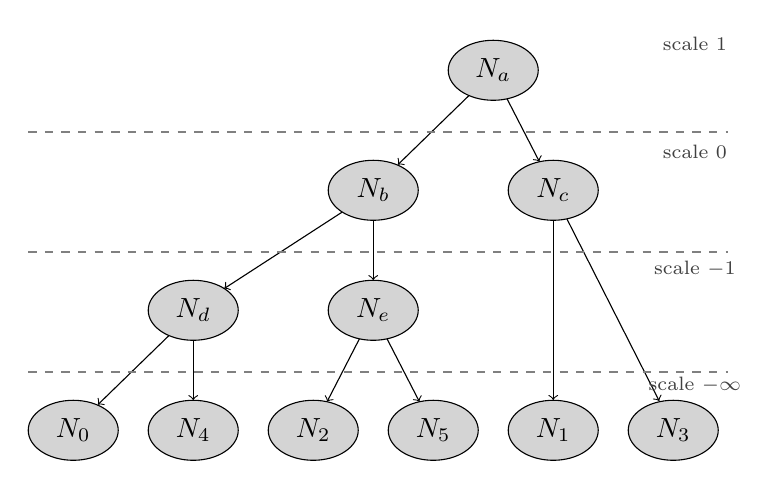
\begin{tikzpicture}[scale=0.6]
      %%
\begin{scope}
  \pgfsetstrokecolor{black}
  \definecolor{strokecol}{rgb}{1.0,1.0,1.0};
  \pgfsetstrokecolor{strokecol}
  \definecolor{fillcol}{rgb}{1.0,1.0,1.0};
  \pgfsetfillcolor{fillcol}
  \filldraw (0bp,0bp) -- (0bp,252bp) -- (414bp,252bp) -- (414bp,0bp) -- cycle;
\end{scope}
\begin{scope}
  \pgfsetstrokecolor{black}
  \definecolor{strokecol}{rgb}{1.0,1.0,1.0};
  \pgfsetstrokecolor{strokecol}
  \definecolor{fillcol}{rgb}{1.0,1.0,1.0};
  \pgfsetfillcolor{fillcol}
  \filldraw (0bp,0bp) -- (0bp,252bp) -- (414bp,252bp) -- (414bp,0bp) -- cycle;
\end{scope}
\begin{scope}
  \pgfsetstrokecolor{black}
  \definecolor{strokecol}{rgb}{1.0,1.0,1.0};
  \pgfsetstrokecolor{strokecol}
  \definecolor{fillcol}{rgb}{1.0,1.0,1.0};
  \pgfsetfillcolor{fillcol}
  \filldraw (0bp,0bp) -- (0bp,252bp) -- (414bp,252bp) -- (414bp,0bp) -- cycle;
\end{scope}
  \pgfsetcolor{black}
  % Edge: ne -> ni
  \draw [->] (215.35bp,72.765bp) .. controls (219.71bp,64.283bp) and (225.15bp,53.714bp)  .. (234.7bp,35.147bp);
  % Edge: nd -> ng
  \draw [->] (99bp,71.697bp) .. controls (99bp,63.983bp) and (99bp,54.712bp)  .. (99bp,36.104bp);
  % Edge: nd -> nf
  \draw [->] (84.43bp,74.834bp) .. controls (74.25bp,64.938bp) and (60.476bp,51.546bp)  .. (41.796bp,33.385bp);
  % Edge: nb -> ne
  \draw [->] (207bp,143.7bp) .. controls (207bp,135.98bp) and (207bp,126.71bp)  .. (207bp,108.1bp);
  % Edge: nc -> nk
  \draw [->] (323.26bp,144.71bp) .. controls (335.67bp,120.23bp) and (359.24bp,73.739bp)  .. (378.62bp,35.537bp);
  % Edge: nb -> nd
  \draw [->] (188.19bp,148.81bp) .. controls (171bp,137.67bp) and (145.38bp,121.06bp)  .. (117.6bp,103.05bp);
  % Edge: na -> nb
  \draw [->] (264.43bp,218.83bp) .. controls (254.25bp,208.94bp) and (240.48bp,195.55bp)  .. (221.8bp,177.38bp);
  % Edge: na -> nc
  \draw [->] (287.35bp,216.76bp) .. controls (291.71bp,208.28bp) and (297.15bp,197.71bp)  .. (306.7bp,179.15bp);
  % Edge: nc -> nj
  \draw [->] (315bp,143.87bp) .. controls (315bp,119.67bp) and (315bp,75.211bp)  .. (315bp,36.189bp);
  % Edge: ne -> nh
  \draw [->] (198.65bp,72.765bp) .. controls (194.29bp,64.283bp) and (188.85bp,53.714bp)  .. (179.3bp,35.147bp);
  % Node: nh
\begin{scope}
  \definecolor{strokecol}{rgb}{0.0,0.0,0.0};
  \pgfsetstrokecolor{strokecol}
  \definecolor{fillcol}{rgb}{0.83,0.83,0.83};
  \pgfsetfillcolor{fillcol}
  \filldraw [opacity=1] (171bp,18bp) ellipse (27bp and 18bp);
  \draw (171bp,18bp) node {$\mathscr{N}_2$};
\end{scope}
  % Node: ni
\begin{scope}
  \definecolor{strokecol}{rgb}{0.0,0.0,0.0};
  \pgfsetstrokecolor{strokecol}
  \definecolor{fillcol}{rgb}{0.83,0.83,0.83};
  \pgfsetfillcolor{fillcol}
  \filldraw [opacity=1] (243bp,18bp) ellipse (27bp and 18bp);
  \draw (243bp,18bp) node {$\mathscr{N}_5$};
\end{scope}
  % Node: nj
\begin{scope}
  \definecolor{strokecol}{rgb}{0.0,0.0,0.0};
  \pgfsetstrokecolor{strokecol}
  \definecolor{fillcol}{rgb}{0.83,0.83,0.83};
  \pgfsetfillcolor{fillcol}
  \filldraw [opacity=1] (315bp,18bp) ellipse (27bp and 18bp);
  \draw (315bp,18bp) node {$\mathscr{N}_1$};
\end{scope}
  % Node: nk
\begin{scope}
  \definecolor{strokecol}{rgb}{0.0,0.0,0.0};
  \pgfsetstrokecolor{strokecol}
  \definecolor{fillcol}{rgb}{0.83,0.83,0.83};
  \pgfsetfillcolor{fillcol}
  \filldraw [opacity=1] (387bp,18bp) ellipse (27bp and 18bp);
  \draw (387bp,18bp) node {$\mathscr{N}_3$};
\end{scope}
  % Node: na
\begin{scope}
  \definecolor{strokecol}{rgb}{0.0,0.0,0.0};
  \pgfsetstrokecolor{strokecol}
  \definecolor{fillcol}{rgb}{0.83,0.83,0.83};
  \pgfsetfillcolor{fillcol}
  \filldraw [opacity=1] (279bp,234bp) ellipse (27bp and 18bp);
  \draw (279bp,234bp) node {$\mathscr{N}_a$};
\end{scope}
  % Node: nb
\begin{scope}
  \definecolor{strokecol}{rgb}{0.0,0.0,0.0};
  \pgfsetstrokecolor{strokecol}
  \definecolor{fillcol}{rgb}{0.83,0.83,0.83};
  \pgfsetfillcolor{fillcol}
  \filldraw [opacity=1] (207bp,162bp) ellipse (27bp and 18bp);
  \draw (207bp,162bp) node {$\mathscr{N}_b$};
\end{scope}
  % Node: nc
\begin{scope}
  \definecolor{strokecol}{rgb}{0.0,0.0,0.0};
  \pgfsetstrokecolor{strokecol}
  \definecolor{fillcol}{rgb}{0.83,0.83,0.83};
  \pgfsetfillcolor{fillcol}
  \filldraw [opacity=1] (315bp,162bp) ellipse (27bp and 18bp);
  \draw (315bp,162bp) node {$\mathscr{N}_c$};
\end{scope}
  % Node: nd
\begin{scope}
  \definecolor{strokecol}{rgb}{0.0,0.0,0.0};
  \pgfsetstrokecolor{strokecol}
  \definecolor{fillcol}{rgb}{0.83,0.83,0.83};
  \pgfsetfillcolor{fillcol}
  \filldraw [opacity=1] (99bp,90bp) ellipse (27bp and 18bp);
  \draw (99bp,90bp) node {$\mathscr{N}_d$};
\end{scope}
  % Node: ne
\begin{scope}
  \definecolor{strokecol}{rgb}{0.0,0.0,0.0};
  \pgfsetstrokecolor{strokecol}
  \definecolor{fillcol}{rgb}{0.83,0.83,0.83};
  \pgfsetfillcolor{fillcol}
  \filldraw [opacity=1] (207bp,90bp) ellipse (27bp and 18bp);
  \draw (207bp,90bp) node {$\mathscr{N}_e$};
\end{scope}
  % Node: nf
\begin{scope}
  \definecolor{strokecol}{rgb}{0.0,0.0,0.0};
  \pgfsetstrokecolor{strokecol}
  \definecolor{fillcol}{rgb}{0.83,0.83,0.83};
  \pgfsetfillcolor{fillcol}
  \filldraw [opacity=1] (27bp,18bp) ellipse (27bp and 18bp);
  \draw (27bp,18bp) node {$\mathscr{N}_0$};
\end{scope}
  % Node: ng
\begin{scope}
  \definecolor{strokecol}{rgb}{0.0,0.0,0.0};
  \pgfsetstrokecolor{strokecol}
  \definecolor{fillcol}{rgb}{0.83,0.83,0.83};
  \pgfsetfillcolor{fillcol}
  \filldraw [opacity=1] (99bp,18bp) ellipse (27bp and 18bp);
  \draw (99bp,18bp) node {$\mathscr{N}_4$};
\end{scope}

\draw[gray,thin,dashed] (0bp,53bp) -- (420bp,53bp);
\draw[gray,thin,dashed] (0bp,125bp) -- (420bp,125bp);
\draw[gray,thin,dashed] (0bp,197bp) -- (420bp,197bp);

\draw (400bp,250bp) node[darkgray] {\scriptsize scale $1$};
\draw (400bp,185bp) node[darkgray] {\scriptsize scale $0$};
\draw (400bp,115bp) node[darkgray] {\scriptsize scale $-1$};
\draw (400bp,45bp) node[darkgray] {\scriptsize scale $-\infty$};

%

    \end{tikzpicture}
  \end{center}
  \vspace*{-0.5em}
  \caption{Abstract representation.}
  \label{fig:cover-tree-ex}
\end{subfigure}
  \vspace*{-0.5em}
\caption{Example cover tree on six points in $\mathcal{R}^2$.  (a)
$\mathscr{N}_a$ is centered at $p_0$ with scale $1$.  (b) $\mathscr{N}_b$ and
$\mathscr{N}_c$ are centered at $p_0$ and $p_1$, respectively, and have scale
$0$.  (c) $\mathscr{N}_d$ and $\mathscr{N}_e$ are centered at $p_0$ and $p_2$,
respectively, and have scale $-1$.  The leaves, $\mathscr{N}_0$ through
$\mathscr{N}_6$, are centered at each of the six points, with scale $-\infty$
(and therefore radius 0).  Note that although node $\mathscr{N}_b$ in subfigure
(b) overlaps node $\mathscr{N}_c$, point $p_1$ only belongs to $\mathscr{N}_c$,
not $\mathscr{N}_b$.  Note also that this is only one valid cover tree that
could be built on the data; other configurations are possible; for instance,
selecting a different root point gives different valid cover trees.}
\label{fig:example-cover-tree}
\end{figure}

\subsection{Expansion constant}

The explicit representation of a cover tree has a number of useful theoretical
properties based on the expansion constant \citep{karger2002finding}; we restate
its definition below.

\begin{defn}
\label{def:int_dim}
Let $B_S(p, \Delta)$ be the set of points in $S$ within a closed ball of radius
$\Delta$ around some $p \in S$ with respect to a metric $d$:
%
$B_S(p, \Delta) = \{ r \in S \colon d(p, r) \leq \Delta \}$.
%
Then, the {\bf expansion constant} of $S$ with respect to the metric $d$ is the
smallest $c \ge 2$ such that

\begin{equation}
| B_S(p, 2 \Delta) | \le c | B_S(p, \Delta) |\ \forall\ p \in S,\
\forall\ \Delta > 0.
\end{equation}

\end{defn}

The expansion constant is used heavily in the cover tree literature.  It is,
in some sense, a notion of instrinic dimensionality, most useful in scenarios
where $c$ is independent of the number of points in the dataset
\citep{karger2002finding, langford2006, krauthgamer2004navigating, ram2009}.
Note also that if points in $S \subset \mathcal{H}$ are being drawn according to
a stationary distribution $f(x)$, then $c$ will converge to some finite value
$c_f$ as $|S| \to \infty$.  To see this, define $c_f$ as a generalization of the
expansion constant for distributions.  $c_f \ge 2$ is the smallest value such
that

\begin{equation}
\int_{\mathcal{B}_{\mathcal{H}}(p, 2 \Delta)} f(x) dx \le c_{f}
\int_{\mathcal{B}_{\mathcal{H}}(p, \Delta)} f(x)
dx
\end{equation}

\noindent for all $p \in \mathcal{H}$ and $\Delta > 0$ such that
$\int_{\mathcal{B}_{\mathcal{H}}(p, \Delta)} f(x) dx > 0$, and with
$\mathcal{B}_{\mathcal{H}}(p, \Delta)$ defined as the closed ball of radius
$\Delta$ in the space $\mathcal{H}$.

As a simple example, take $f(x)$ as a uniform spherical distribution in
$\mathcal{R}^d$: for any $|x| \le 1$, $f(x)$ is a constant; for $|x| > 1$, $f(x)
= 0$.  It is easy to see that $c_f$ in this situation is $2^d$, and thus for
some dataset $S$, $c$ must converge to that value as more and more points are
added to $S$.  Closed-form solutions for $c_f$ for more complex distributions
are less easy to derive; however, empirical speedup results from
\citet{langford2006} suggest the existence of datasets where $c$ is not strongly
dependent on $d$.  For instance, the \texttt{covtype} dataset has 54 dimensions
but the expansion constant is much smaller than other, lower-dimensional
datasets.
% To demonstrate this convergence, Table
%\ref{tab:ec_scaling} shows results for 10 trials of empirically calculated
%expansion constants for datasets drawn from this distribution, for varying $d$.

%\begin{table}[htb]
%\begin{center}
%\begin{tabular}{|l|c|c|c|c|}
%\hline
%$|S|$ & $d = 2$ & $d = 5$ & $d = 10$ & $d = 20$ \\
%\hline
%10      & 6     & 10    & 10    &         \\
%31      & 12    & 31    & 31    &         \\
%100     & 13    & 64    & 100   &         \\
%316     & 23    & 96    & 286   &         \\
%1000    & 26    & 126   & 673   &         \\
%3162    & 29    & 189   & 1348  &         \\
%10000   & 30    & 259   & 2646  &         \\
%31622   & 39    & 309   & 3858  &         \\
%100000  & 40    & 360   & 7162  &         \\
%316227  & 46    & 385   & 8297  &         \\
%1000000 &       &       &       &         \\
%$\infty$ ($c_f$)   & 4     & 32    & 1024  & 1048576 \\
%\hline
%\end{tabular}
%\end{center}
%\caption{Calculated $c$ for uniform hypersphere distribution as
%$|S|$ scales.}
%\label{tab:ec_scaling}
%\end{table}

%We are somewhat limited in the sizes of $|S|$ we can scale to, because
%calculating the expansion constant of a dataset is a computationally intensive
%task.  Nonetheless, we can see that the expansion constant moves towards the
%final value of $c_f$, though potentially from above ({\it The results are not
%done yet.  This paragraph may need rewriting.  But I strongly suspect the
%results will show what I've said.}).  We postulate that the behavior of more
%complex real-world datasets is similar.

There are some other important observations about the behavior of $c$.  Adding a
single point to $S$ may increase $c$ arbitrarily: consider a set $S$ distributed
entirely on the surface of a unit hypersphere.  If one adds a single point at
the origin, producing the set $S'$, then $c$ explodes to $|S'|$ whereas before
it may have been much smaller than $|S|$.  Adding a single point may also
decrease $c$ significantly.  Suppose one adds a point arbitrarily close to the
origin to $S'$; now, the expansion constant will be $|S'| / 2$.  Both of these
situations are degenerate cases not commonly encountered in real-world behavior;
we discuss them in order to point out that although we can bound the behavior of
$c$ as $|S| \to \infty$ for $S$ from a stationary distribution, we are not able
to easily say much about its convergence behavior.

The expansion constant can be used to show a few useful bounds on various
properties of the cover tree; we restate these results below, given some cover
tree built on a dataset $S$ with expansion constant $c$ and $|S| = N$:

\begin{itemize}
  \item {\bf Width bound:} no cover tree node has more than $c^4$ children
(Lemma 4.1, \cite{langford2006}).

  \item {\bf Depth bound:} the maximum depth of any node is $O(c^2 \log N)$
(Lemma 4.3, \cite{langford2006}).

  \item {\bf Space bound:} a cover tree has $O(N)$ nodes (Theorem 1,
\cite{langford2006}).
\end{itemize}

%\begin{lemma}
%\label{lem:width}
%(Lemma 4.1, \cite{langford2006}) The number of children of any cover tree node $\mathscr{N}_i$ is bounded by
%$c^4$, where $c$ is the expansion constant of the dataset the cover tree is
%built on, as defined in Definition \ref{def:int_dim}.
%\end{lemma}

%\begin{lemma}
%\label{lem:depth}
%(Lemma 4.3, \cite{langford2006}) The maximum depth of any point $p_r$ in a cover
%tree $\mathscr{T}_r$ is $O(c^2 \log N)$, where $N$ is the number of points in
%the dataset that $\mathscr{T}_r$ is built on.
%\end{lemma}

Lastly, we introduce a convenience lemma of our own which is a generalization of
the packing arguments used by \citet{langford2006}.  This is a more flexible
version of their argument.

\begin{lemma}
Consider a dataset $S$ with expansion constant $c$ and a subset $C \subseteq S$
such that every point in $C$ is separated by $\delta$.  Then, for any point
$p$ (which may or may not be in $S$), and any radius $\rho \delta > 0$:
\begin{equation}
| B_S(p, \rho \delta) \cap C | \le c^{2 + \lceil \log_2 \rho \rceil}.
\end{equation}
\label{lem:packing}
\end{lemma}

\begin{proof}
The proof is based on the packing argument from Lemma 4.1 in
\cite{langford2006}. Consider two cases: first, let $d(p, p_i) > \rho \delta$
for any $p_i \in S$. In this case, $B_S(p, \rho \delta) = \emptyset$ and the
lemma holds trivially.
Otherwise, let $p_i \in S$ be a point such that $d(p, p_i) \leq \rho \delta$.
Observe that $B_S(p, \rho \delta) \subseteq B_S(p_i, 2 \rho \delta)$.
Also, $| B_S(p_i, 2 \rho \delta) | \le c^{2 + \lceil \log_2 \rho
\rceil} | B_S(p_i, \delta / 2) |$ by the definition of the expansion constant.
Because each point in $C$ is separated by $\delta$, the
number of points in $B_S(p, \rho \delta) \cap C$ is
bounded by the number of disjoint balls of radius $\delta / 2$ that can be
packed into $B_S(p, \rho \delta)$.  In the worst case, this packing is
perfect, and

\begin{equation}
|B_S(p, \rho \delta)| \le \frac{|B_S(p_i, 2 \rho \delta)|}{|B_S(p_i, \delta
/ 2)|} \le c^{2 + \lceil \log_2 \rho \rceil}.
\end{equation}
\end{proof}
